% Chapter 7: Security
\chapter{Security Layer}

\section{Overview}

The security layer implements JWT-based authentication and role-based authorization using Spring Security 6.x (Spring Boot 3.2.0).

\section{SecurityConfig}

\subsection{Complete Source Code}

\begin{lstlisting}[caption=SecurityConfig.java]
@Configuration
@EnableWebSecurity
@EnableMethodSecurity
public class SecurityConfig {

    @Autowired
    private JwtRequestFilter jwtRequestFilter;

    @Value(''${cors.allowed-origins}'')
    private String allowedOrigins;

    @Bean
    public SecurityFilterChain securityFilterChain(
            HttpSecurity http) throws Exception {
        http
            .cors(cors -> cors.configurationSource(
                corsConfigurationSource()))
            .csrf(csrf -> csrf.disable())
            .authorizeHttpRequests(auth -> auth
                .requestMatchers(''/api/auth/**'').permitAll()
                .requestMatchers(''/swagger-ui/**'', 
                    ''/v3/api-docs/**'', 
                    ''/swagger-ui.html'').permitAll()
                .requestMatchers(''/api/admin/**'').hasRole(''ADMIN'')
                .requestMatchers(''/api/candidate/**'')
                    .hasRole(''CANDIDATE'')
                .anyRequest().authenticated()
            )
            .sessionManagement(session -> session
                .sessionCreationPolicy(SessionCreationPolicy.STATELESS))
            .addFilterBefore(jwtRequestFilter, 
                UsernamePasswordAuthenticationFilter.class);

        return http.build();
    }

    @Bean
    public CorsConfigurationSource corsConfigurationSource() {
        CorsConfiguration configuration = new CorsConfiguration();
        configuration.setAllowedOrigins(
            List.of(allowedOrigins.split('','')));
        configuration.setAllowedMethods(
            Arrays.asList(''GET'', ''POST'', ''PUT'', ''DELETE'', ''OPTIONS''));
        configuration.setAllowedHeaders(Arrays.asList(''*''));
        configuration.setAllowCredentials(true);
        
        UrlBasedCorsConfigurationSource source = 
            new UrlBasedCorsConfigurationSource();
        source.registerCorsConfiguration(''/**'', configuration);
        return source;
    }

    @Bean
    public PasswordEncoder passwordEncoder() {
        return new BCryptPasswordEncoder();
    }
}
\end{lstlisting}

\subsection{Line-by-Line Explanation}

\begin{itemize}[leftmargin=*]
    \item \textbf{@Configuration}: Marks as Spring configuration class
    \item \textbf{@EnableWebSecurity}: Enables Spring Security
    \item \textbf{@EnableMethodSecurity}: Enables method-level security annotations
    
    \item \textbf{SecurityFilterChain Bean}
    \begin{itemize}
        \item Configures HTTP security using lambda DSL (Spring Security 6.x style)
        \item Replaces deprecated \texttt{WebSecurityConfigurerAdapter}
    \end{itemize}
    
    \item \textbf{CORS Configuration}
    \begin{itemize}
        \item Enables Cross-Origin Resource Sharing
        \item References custom configuration source
    \end{itemize}
    
    \item \textbf{CSRF Disabled}
    \begin{itemize}
        \item Cross-Site Request Forgery protection disabled
        \item Safe for stateless JWT authentication
        \item Required for REST APIs
    \end{itemize}
    
    \item \textbf{Authorization Rules}
    \begin{itemize}
        \item \texttt{/api/auth/**}: Public (login endpoint)
        \item \texttt{/swagger-ui/**}: Public (API documentation)
        \item \texttt{/api/admin/**}: Requires ADMIN role
        \item \texttt{/api/candidate/**}: Requires CANDIDATE role
        \item All other requests: Authenticated users only
    \end{itemize}
    
    \item \textbf{Session Management}
    \begin{itemize}
        \item \texttt{STATELESS}: No HTTP sessions created
        \item Each request authenticated independently via JWT
        \item Enables horizontal scalability
    \end{itemize}
    
    \item \textbf{JWT Filter}
    \begin{itemize}
        \item Added before \texttt{UsernamePasswordAuthenticationFilter}
        \item Processes JWT token from Authorization header
        \item Sets authentication in SecurityContext
    \end{itemize}
    
    \item \textbf{CORS Configuration Source}
    \begin{itemize}
        \item Reads allowed origins from properties
        \item Supports multiple origins (comma-separated)
        \item Allows all HTTP methods needed for REST
        \item Allows credentials (cookies, auth headers)
    \end{itemize}
    
    \item \textbf{PasswordEncoder Bean}
    \begin{itemize}
        \item BCrypt algorithm for password hashing
        \item Automatically salted
        \item Adjustable strength factor
    \end{itemize}
\end{itemize}

\section{JwtUtil}

\subsection{Purpose}
Utility class for JWT token generation, parsing, and validation using JJWT library.

\subsection{Key Methods}

\begin{lstlisting}[caption=JWT Token Generation]
public String generateToken(String email, String role) {
    Map<String, Object> claims = new HashMap<>();
    claims.put(''role'', role);
    return createToken(claims, email);
}

private String createToken(Map<String, Object> claims, 
                          String subject) {
    return Jwts.builder()
            .setClaims(claims)
            .setSubject(subject)
            .setIssuedAt(new Date(System.currentTimeMillis()))
            .setExpiration(new Date(System.currentTimeMillis() 
                + expiration))
            .signWith(getSigningKey(), SignatureAlgorithm.HS512)
            .compact();
}
\end{lstlisting}

\textbf{Token Structure:}
\begin{itemize}
    \item \textbf{Claims:} Custom data (role)
    \item \textbf{Subject:} User email
    \item \textbf{Issued At:} Token creation time
    \item \textbf{Expiration:} Configurable (24 hours default)
    \item \textbf{Signature:} HMAC-SHA512 algorithm
\end{itemize}

\begin{lstlisting}[caption=JWT Token Extraction]
public String extractEmail(String token) {
    return extractClaims(token).getSubject();
}

public String extractRole(String token) {
    return extractClaims(token).get(''role'', String.class);
}

private Claims extractClaims(String token) {
    return Jwts.parserBuilder()
            .setSigningKey(getSigningKey())
            .build()
            .parseClaimsJws(token)
            .getBody();
}
\end{lstlisting}

\begin{lstlisting}[caption=JWT Token Validation]
public Boolean isTokenValid(String token) {
    try {
        Jwts.parserBuilder()
                .setSigningKey(getSigningKey())
                .build()
                .parseClaimsJws(token);
        return !isTokenExpired(token);
    } catch (Exception e) {
        return false;
    }
}

public Boolean isTokenExpired(String token) {
    return extractExpiration(token).before(new Date());
}
\end{lstlisting}

\textbf{Validation Checks:}
\begin{itemize}
    \item Signature verification
    \item Expiration check
    \item Format validation
    \item Exception handling for malformed tokens
\end{itemize}

\section{JwtRequestFilter}

\subsection{Purpose}
Filter that intercepts every request to extract and validate JWT tokens, setting authentication context.

\subsection{Complete doFilterInternal Method}

\begin{lstlisting}[caption=JWT Request Filter Logic]
@Override
protected void doFilterInternal(HttpServletRequest request, 
                               HttpServletResponse response, 
                               FilterChain chain)
        throws ServletException, IOException {

    final String authorizationHeader = 
        request.getHeader(''Authorization'');

    String email = null;
    String jwt = null;

    if (authorizationHeader != null && 
        authorizationHeader.startsWith(''Bearer '')) {
        jwt = authorizationHeader.substring(7);
        
        try {
            if (!jwtUtil.isTokenValid(jwt)) {
                response.setStatus(
                    HttpServletResponse.SC_UNAUTHORIZED);
                response.setContentType(''application/json'');
                response.getWriter().write(
                    ''{\''error\'': \''Invalid or expired token\''}'');
                return;
            }
            
            email = jwtUtil.extractEmail(jwt);
            String role = jwtUtil.extractRole(jwt);

            if (email != null && SecurityContextHolder
                    .getContext().getAuthentication() == null) {
                UsernamePasswordAuthenticationToken authToken = 
                    new UsernamePasswordAuthenticationToken(
                        email, null, Collections.singletonList(
                            new SimpleGrantedAuthority(
                                ''ROLE_'' + role)));
                authToken.setDetails(
                    new WebAuthenticationDetailsSource()
                        .buildDetails(request));
                SecurityContextHolder.getContext()
                    .setAuthentication(authToken);
            }
        } catch (Exception e) {
            logger.error(''JWT validation failed: '' + e.getMessage());
            response.setStatus(HttpServletResponse.SC_UNAUTHORIZED);
            response.setContentType(''application/json'');
            response.getWriter().write(
                ''{\''error\'': \''Invalid token: '' + 
                e.getMessage() + ''\''}'');
            return;
        }
    }

    chain.doFilter(request, response);
}
\end{lstlisting}

\subsection{Processing Flow}

\begin{enumerate}
    \item Extract Authorization header
    \item Check for ''Bearer '' prefix
    \item Extract JWT token (remove ''Bearer '' prefix)
    \item Validate token signature and expiration
    \item If invalid, return 401 Unauthorized and stop
    \item Extract email and role from token
    \item Create \texttt{UsernamePasswordAuthenticationToken}
    \item Add role as \texttt{SimpleGrantedAuthority} with ''ROLE\_'' prefix
    \item Set authentication in \texttt{SecurityContext}
    \item Continue filter chain
\end{enumerate}

\subsection{Security Context}

\textbf{Authentication Object Contents:}
\begin{itemize}
    \item \textbf{Principal:} User email (username)
    \item \textbf{Credentials:} null (JWT is stateless)
    \item \textbf{Authorities:} List with single role (ROLE\_ADMIN or ROLE\_CANDIDATE)
    \item \textbf{Details:} Request details (IP, session ID, etc.)
\end{itemize}

\section{Authentication Flow Diagram}

\begin{figure}[h]
\centering
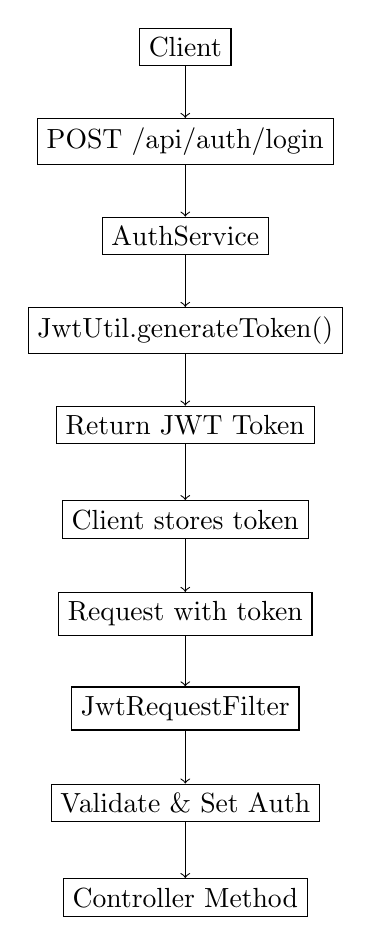
\begin{tikzpicture}[node distance=1.2cm]
    \node[draw, rectangle] (client) {Client};
    \node[draw, rectangle, below of=client] (login) {POST /api/auth/login};
    \node[draw, rectangle, below of=login] (authservice) {AuthService};
    \node[draw, rectangle, below of=authservice] (jwtutil) {JwtUtil.generateToken()};
    \node[draw, rectangle, below of=jwtutil] (response) {Return JWT Token};
    \node[draw, rectangle, below of=response] (store) {Client stores token};
    \node[draw, rectangle, below of=store] (request) {Request with token};
    \node[draw, rectangle, below of=request] (filter) {JwtRequestFilter};
    \node[draw, rectangle, below of=filter] (validate) {Validate \& Set Auth};
    \node[draw, rectangle, below of=validate] (controller) {Controller Method};
    
    \draw[->] (client) -- (login);
    \draw[->] (login) -- (authservice);
    \draw[->] (authservice) -- (jwtutil);
    \draw[->] (jwtutil) -- (response);
    \draw[->] (response) -- (store);
    \draw[->] (store) -- (request);
    \draw[->] (request) -- (filter);
    \draw[->] (filter) -- (validate);
    \draw[->] (validate) -- (controller);
\end{tikzpicture}
\caption{Complete Authentication Flow}
\end{figure}

\section{JWT Token Example}

\subsection{Token Structure}

A JWT consists of three parts separated by dots:

\texttt{header.payload.signature}

\textbf{Header (Base64):}
\begin{lstlisting}[language=json]
{
  ''alg'': ''HS512'',
  ''typ'': ''JWT''
}
\end{lstlisting}

\textbf{Payload (Base64):}
\begin{lstlisting}[language=json]
{
  ''role'': ''ADMIN'',
  ''sub'': ''admin@quizforge.com'',
  ''iat'': 1699632000,
  ''exp'': 1699718400
}
\end{lstlisting}

\textbf{Signature:}
\begin{lstlisting}
HMACSHA512(
  base64UrlEncode(header) + ''.'' + base64UrlEncode(payload),
  secret
)
\end{lstlisting}

